In this section, we will discuss the \texttt{4Ps Marketing Mix} of our research product \emph{(Google Stadia)}. We will discuss the product definition, its price analysis, its place and promotion. This helps us further understand the marketing setup of this new product and develop a common understand of how it begins and whether it will stand and succeed.

\begin{figure}[h]
    \centering
    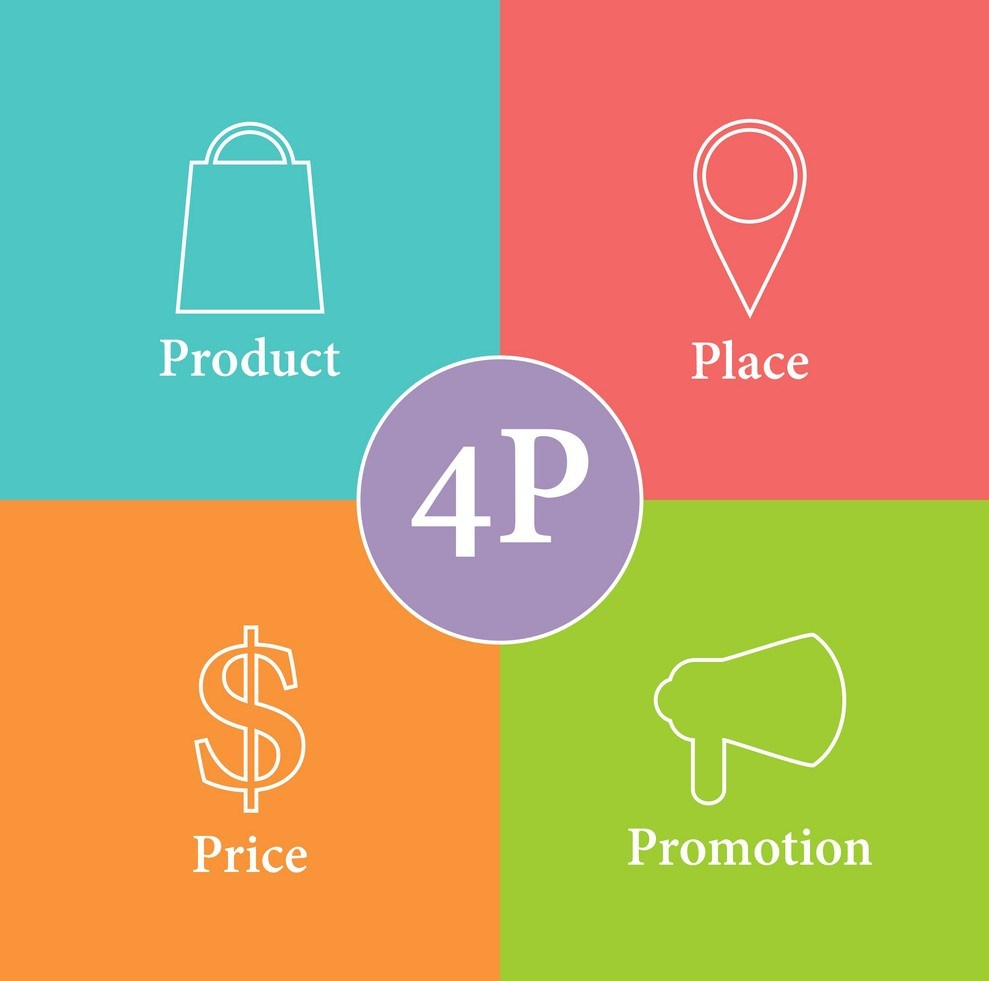
\includegraphics[width=0.5\textwidth]{images/4p.jpg}
    \caption{4Ps Marketing Mix Diagram}
    \label{fig:4p}
\end{figure}

\subsection{Product}
As mentioned before, \emph{Google Stadia} is a cloud streaming service for video games, where gamers can stream video games, running on cloud systems, without having to buy the game console themselves. Stadia offers a very cheap way of playing videos games for gamers, who can't afford buying a game console or an expensive gaming rig. \\

To use Stadia service, the user just need a device with \emph{Google Chrome} or any Stadia-supported application on his/her personal computer or mobile phone and a reliable internet connection, in addition to the monthly subscription. \\

Stadia is not the first project of its kind. We have \emph{Nvidia Geforce Now} and \emph{Microsoft Project XCloud}. However, Stadia offers seamless $4K$ video game streaming based on \emph{Youtube} streaming service, which is a big bonus over other streaming services. 

\subsection{Price}
Stadia is subscription-based service, where the users pay a monthly fee, in order to use the service. There are two levels of membership: \emph{Stadia Pro}, which is paid for, and \emph{plain Stadia}, a free access plan. \\

\emph{Stadia Pro} offers the user a seamless $HDR$ $4K$ gaming experience, with a good library of video games. However, the user still has to purchase most of the video games on top of it. Stadia Pro membership costs $8.99$ $GBP$ per month in the UK, $\$9.99$ $USD$ per month in the US. New subscribers can get a free one-month trial of Pro membership. \\

The alternative plan is \emph{plain Stadia} (a.k.a. Stadia Base). In this plan, users must purchase any required video game themselves. Also, the streaming quality is limited to $1080p$. This comes with an advantage that user doesn't have to pay any monthly fee.

\subsection{Place}
Since Stadia is an online cloud streaming platform, it's available worldwide. It's unavailable only in \emph{Hawaii} and \emph{Guam}. However, such service can be unpopular in countries, where internet connectivity is limited, such as African countries.

\subsection{Promotion}
\texttt{Google} follows an online promotion campaign, through advertisement on online platforms such as \emph{Youtube}. Most of the details of the platform development can be found at their developers website \cite{stadia_website}. Open source contribution to the project is also applicable.  \\

The service also provides a one-month free trial for Pro membership to encourage different users to use their platform. \texttt{Google} is also enhancing the service by including more video games and improving the streaming performance.